\chapter{Background}
\label{background}

In this section we will provide a brief tour of the OCaml programming
language, focusing espectially on its powerful module system. The
chapter follows with a discussion of xUnit's Test Double patterns and
their implementation in OCaml and Java. The chapter concludes with a
summary of the current state-of-the-art testing tools for functional
languages such as OCaml and Haskell.

\section{A brief tour of OCaml and its module system}
\label{ocaml}

%% XXX TODO: define commands to change settings for java and for ocaml

%% https://tex.stackexchange.com/questions/106844/adding-words-to-lstlisting-for-python-langaue
%% in order to get multiple levels of keywords
\lstset{
  language=ML,
  morekeywords={function,module,match,try},
  % XXX fix top/bottom frame margin spacing
  % https://tex.stackexchange.com/questions/31598/lstlisting-produces-empty-row-when-used-inside-a-tabular
  aboveskip=-\baselineskip,
  %% framextopmargin=0pt,
  %% framexbottommargin=10pt,
  %% belowskip=10pt,
}

%% Want to talk quickly about code (functions, types, type inference),
%% modules, functors, first class modules. Mention that OCaml has a class
%% language, but that idiomatic OCaml typically uses functions and
%% modules unless a particular algorithm or solution to a problem
%% warrants an object-oriented implemtation.

OCaml is a strongly, statically typed functional programming language
based on the ML family of languages. It may be interpreted in a
read-eval-print loop called the OCaml ``toplevel,'' or it may be
compiled to an OCaml specific bytecode languate or to a native
executable. \cite{ocaml:spec} It has a very good generational garbage
collector tuned for sequential programs. \cite{ocaml:gc_tutorial}

What follows is a \textit{very} brief tour of the OCaml programming
language. This should hopefully be enough to allow the reader to
follow along with the coding examples later in this chapter and the
next. For more assistance with OCaml, the reader is directed to the
OCaml Langauge Specification \cite{ocaml:spec}, and Real World OCaml
\cite{rwo}\footnote{Real World OCaml is available for free online:
  \url{https://realworldocaml.org}}

\subsection{OCaml basics: values, functions, and types}

\subsubsection{Values}

In OCaml, values are assigned to variables using the \code{let}
keyword.

\begin{lstlisting}
(* This is a comment *)
let num = 42
let str = "hello world"
let list = [1;2;3;4]
let tuple = (1,2)
\end{lstlisting}

Variables in OCaml are immutable, unless they are specially defined as
references, or mutable fields of a record type.

\begin{lstlisting}
let num = ref 42
Printf.printf "num was %d\n" !num
num := 24
Printf.printf "num is now %d\n" !num
\end{lstlisting}

\subsubsection{Functions}

Functions are created with the keywords \code{fun} or \code{function},
and assigned names using \code{let}, just like other values. Functions
defined using the \code{function} keyword can only take one arguement,
but that argument can be pattern-matched.

\begin{lstlisting}
let f = fun a b -> a + b
let g = function
        | [] -> true
        | _  -> false
\end{lstlisting}

Functions can also be created using a shorthand \code{let} syntax. The
function \code{f} below is equivalent to the function \code{f} above.

\begin{lstlisting}
let f a b = a + b
\end{lstlisting}

Because functions are first-class values just like \code{int}s and
\code{string}s, we can pass them to other functions. For instance, the
function \code{List.map} takes a function \code{f} and a list
\code{ls}, and returns a new list containing the result of applying
\code{f} to each element of \code{ls}.

\begin{lstlisting}
let f x = x + 1
let ls = [1;2;3;4]
List.map f ls         (* returns the value [2;3;4;5] *)
\end{lstlisting}

\subsubsection{Types}

OCaml is a strongly, statically typed language. The compiler will
infer the type of values, and will return an error if a type
constraint is violated. For instance, the following function \code{f}
has type \code{int -> int -> int}, meaning that it takes two values of
type \code{int} and returns a value of type \code{int}. If a
\code{string} or \code{float} are passed to this function, a
compilation error is thrown.

\begin{lstlisting}
let f a b = a + b     (* has type int -> int -> int *)
f 40 2                (* this type-checks *)
f "4" "2"             (* this fails to type-check *)
f 41.8 0.2            (* this also fails to type-check *)
\end{lstlisting}

OCaml allows the user to define complex types.

\begin{lstlisting}
(* Tuples *)
type position = int * int

(* Variant types *)
type colors =
  | Red of int
  | Green of int
  | Blue of int

(* Record types *)
type book = {
  author : string;
  title  : string;
  mutable inventory : int;
}
\end{lstlisting}

%% type variables

Polymorphism in OCaml data types is expressed with type variables. In
the following example, \code{'a} is a type variable which can
represent any type, making \code{tree} a generic data type.

\begin{lstlisting}
type 'a tree =
  | Leaf of 'a
  | Node of 'a tree * 'a tree
\end{lstlisting}

\subsubsection{Polymorphic variants}

OCaml has a feature called \emph{polymorphic variants}. These are
similar to atoms or symbols in languages like Erlang or
Scheme. Polymorphic variants are distinguished from regular variants
by the backtick (\code{`}) preceeding the label. Unlike regular
variants, polymorphic variants do not need to be capitalised, but this
is still common practice. A common use of polymorphic variants is to
encode inputs or outputs of functions; for instance, the below
function uses polymorphic variants for encoding success and failure
cases.

\begin{lstlisting}
let f = function
  | `String v ->
    Printf.printf "Got a string: %s\n" v;
     `Success
  | `Int v    ->
    Printf.printf "Got an int: %s\n" v;
    `Success
  | `Float _  ->
    print_endline "Wasn't expecting a float.";
    `Failure
\end{lstlisting}

Polymorphic variants can be used in the same way as regular variant
types, except that they don't need to be explicitly
declared. Furthermore, any polymorphic variant with the same name is
considered to be the same type (unlike regular variants, where
identically named constructors may be protected inside of different
modules, and therefore would be different types).

This gives rise to useful patterns in API development, such as
extensible API types. For instance, the Yojson library has an encoding
of standard JSON, as well as common, useful extensions to the JSON
spec. The standard JSON spec is encoded in \code{Yojson.Basic.json},
whereas the extensions to the standard are encoded in
\code{Yojson.Safe.json}. The \code{json} type in both modules uses
polymorphic variants to define the json grammar, and ``Basic'' JSON
can be easily upgraded to ``Safe'' JSON. A full treatment of this
library can be found in Chapter 15 of Real World OCaml \cite{rwo}.

\subsubsection{Pattern matching}

One of the most powerful features of languages like OCaml is pattern
matching. OCaml allows one to match over the structure of defined data
types. Pattern matching can be accomplished with the
\code{match value with | patt -> expr}
expression, or in functions created with the \code{function}
keyword. The following two functions are equivalent.

\begin{lstlisting}
let rec num_leaves_1 = function
  | Leaf _      -> 1
  | Node (l, r) ->
    (num_leaves l) + (num_leaves r)

let rec num_leaves_2 tr =
  match tr with
  | Leaf _      -> 1
  | Node (l, r) ->
    (num_leaves l) + (num_leaves r)
\end{lstlisting}

Note the use of the underscore (\code{_}) in the \code{Leaf}
pattern. In OCaml, underscore means ``match anything.'' It can also be
used in variable assignment, and is often used in module
initialisation code.

\subsubsection{Exceptions}

OCaml has exceptions that follow the usual ``try/catch''
pattern. OCaml exceptions have no ``finally'' clause, but this can be
implemented in a library using first-class
functions.\footnote{cf. \code{protect} and \code{protectx} in Jane
  Street's Core library:
  \url{https://ocaml.janestreet.com/ocaml-core/111.03.00/doc/core/#Exn}}
Exceptions are declared similarly to variant data types.

\begin{lstlisting}
exception Not_found
let rec find x = function
  | [] -> raise Not_found
  | (k,v)::ls -> if x = k
                 then v
                 else find x ls
\end{lstlisting}

As with variants, exceptions can also carry data:

\begin{lstlisting}
exception Failure of string
exception Error of [`Invalid_request of string | `Permissions]
raise (Error (`Invalid_request "foo"))
raise (Error `Permissions)
\end{lstlisting}

``try/catch'' blocks in OCaml are similar to those in other languages,
except OCaml pattern matches on the ``catch'' block using the
\code{with} keyword.

\begin{lstlisting}
try
  raise (Error (`Invalid_request "foo"))
with
  | Error `Permissions ->
    print_endline "Bad permissions"
  | Error (`Invalid_request req) ->
    Printf.printf "Invalid request: %s\n" req
\end{lstlisting}

\subsection{The OCaml module system}

\subsubsection{Modules, signatures, and compilation units}

A distinguishing feature of OCaml is its powerful module system. A
module in OCaml is the basic compilation unit. Each compiled file is
assigned its own module. For instance, the definitions inside a file
called \code{foo.ml} would be placed into a module \code{Foo}.

%% XXX not sure if we want these to come from separate files, or if we
%% want to put a border around them, or...
%% \lstinputlisting[
%%   caption=foo.ml,
%%   %frame=single,
%% ]{code/foo.ml}
\begin{lstlisting}
type t = int
let f a = a
\end{lstlisting}

From outside of this module, function \code{f} would be referenced as
\code{Foo.f}. Module \code{Foo} has the following type:

\begin{lstlisting}
type t = int
val f : 'a -> 'a
\end{lstlisting}

The types of modules can be restricted useing \code{mli} files. When
an \code{mli} file exists with the same basename as an \code{ml} file,
the module type of the module created for that \code{ml} file is
restricted to that of the signature specified in the \code{mli}
file. For instance, if \code{foo.mli} is:

%\lstinputlisting[caption=foo.mli]{code/foo.mli}
\begin{lstlisting}
type t = int
val f : ’a -> ’a
\end{lstlisting}

then the resulting type of module \code{Foo} would be:

\begin{lstlisting}
type t
val f : t -> t
\end{lstlisting}

Notice that \code{type t} is now abstract (meaning that we can't know
its implementation outside of module \code{Foo}, and function \code{f}
is now restricted to have type \code{t -> t}, instead of the more
general \code{'a -> 'a}.

OCaml modules can also be defined independently of compilation
units.

\begin{lstlisting}
module Bar =
struct
  type t = int
  let g a = a + 1
  let h ls = List.map g ls
end
\end{lstlisting}

We can also create module type signatures, which can restrict the
resulting type of a module in the same way as an \code{mli} file.

\begin{lstlisting}
module type BAR =
sig
  type t
  val h : int list -> int list
end
\end{lstlisting}

We can limit the type of \code{module Bar} to the signature
\code{BAR} by restricting it:

\begin{lstlisting}
module Bar2 = (Bar : BAR)
\end{lstlisting}

We can also restrict the orignal definition of \code{module Bar}:

\begin{lstlisting}
module Bar1 : BAR =
struct
  type t = int
  let g a = a + 1
  let h ls = List.map g ls
end
\end{lstlisting}

Modules \code{Bar1} and \code{Bar2} are now restricted by the
signature \code{BAR}. The value \code{g} is now hidden, and
\code{type t} is now abstract.

\subsubsection{Functors}

In most languages, a module system is primarily meant to provide a
namespacing system or a way to refer to compilation units
(cf. Haskell's module system \cite{www:haskell:modules}, or Python's
module system \cite{www:python:modules}). OCaml, however, has a much
more powerful module system, including the ability to define
\textit{functors}.

A functor is a relation from modules to modules. A functor can take a
module as an arguement, and use it to specialise another module. For
instance, here is an example adapted from the OCaml language
``Introduction to OCaml'' \cite{ocaml:spec} that creates a \code{Set}
functor.

\begin{lstlisting}
module type ORDERED_TYPE =
sig
  type t
  val compare: t -> t -> int
end

module Set =
  functor (Elt: ORDERED_TYPE) ->
    struct
      type element = Elt.t
      type set = element list
      let empty = []
      let add x s = ...
    end
\end{lstlisting}

\code{Set} is a functor that takes some module with same type
signature as \code{ORDERED_TYPE}, and returns a module which is
specialised with that element type. For instance, we may create a new
\code{StringSet} module using the \code{Set} functor and the
\code{String} module from the OCaml standard library.

\begin{lstlisting}
module StringSet = Set(String)

let set = StringSet.add "foo" StringSet.empty in
StringSet.mem "foo" set  (* => true *)
\end{lstlisting}

For brevity, OCaml supports and alternative syntax for functor
definition which is more concise. For instance, we could have defined
the \code{Set} functor as:
\code{module Set(Elt : ORDERED_TYPE) = struct ... end}.
This comes in handy when one is defining a functor which takes
multiple arguements:
\code{module F(A : X)(B : Y) = struct ... end} .

Functors are useful for creating generic data types, such as the
\code{Set} type we defined above. We will soon see that they can also
be useful for dependency injection.

\subsubsection{First-class modules}

OCaml 4.00 introduced the feature of \textit{first-class modules}. A
first-class module is analogous to a language having first-cass
functions: a module in OCaml can be packaged into a value, passed to
functions, and returned from functions. First-class modules provide a
similar capability as functors do, but are much more
light-weight. Refactoring a module into a functor can be a significant
amount of work, but adding a module arguement to a function is a much
simpler change.

\begin{lstlisting}
module type DATABASE = sig ... end

module Db = struct ... end

let f db =
  (* Turn a module value into a module *)
  let module Db = (val db : DATABASE) in
  ...

(* And convert a module into a value *)
let _ = f (module Db : DATABASE)
\end{lstlisting}

\subsection{The rest of OCaml}

%% Briefly mention OCaml's object system and class language, and point
%% the reader to books and web resources.

In additon to the module language described above, OCaml also has a
rich class language and object system. Object orientation is a useful
addition to OCaml, but most OCaml code in practice eschews the use of
objects and classes. This dissertation will ignore the object oriented
features of OCaml and instead focus on its functional core and module
system. Most of the literature regarding software testing assumes
an object oriented implementation langauge; this dissertations
contributions lie elsewhere.

This was a whirlwind tour of OCaml. It was meant to cover just enough
syntax to get the reader through the OCaml examples in the next
section, and to understand the implmentation in the following
chapter. For more extensive coverage, please see the OCaml language
spec \cite{ocaml:spec}, and the excellent Real World OCaml book
\cite{rwo}.

\section{Test Double patterns in detail}
\label{testdoubles}

\begin{figure}
  \centering
  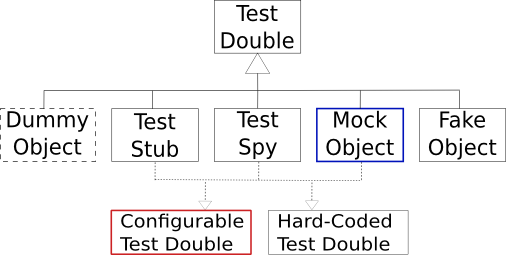
\includegraphics[scale=0.7]{img/test_double_taxonomy.png}
  \caption[Taxonomy of Test Double patterns]{Taxonomy of Test Double patterns\footnotemark}
  \label{fig:taxonomy}
\end{figure}
\footnotetext{Adapted from Meszaros \cite{meszaros:xunit}}

%%% (XXX) As figure \ref{fig:taxonomy} shows\dots

\begin{table}
  \centering
  \begin{tabular}{c|c|c|c|c}
    %% Header
    & Implements Interface
    & Indirect Inputs
    & Indirect Outputs
    & Configurable
    \\ \hline
    %% Rows
    \textit{Dummy} & No & No & No & No \\ \hline
    Stub & Yes & Yes & No & Yes        \\ \hline
    Fake & Yes & No & No & N/A         \\ \hline
    Spy & Yes & No & Yes & Yes         \\ \hline
    Mock & Yes & Yes & Yes & Yes       \\ \hline
  \end{tabular}
  \caption{Foo}
  \label{table:testdoubles}
\end{table}

Test Doubles allow developers to write tests that might have been
difficult or even impossible to write without a Test Double. As their
name suggests, Test Doubles are meant to stand in for a DOC of the
SUT. Their name is analogous to ``stunt doubles'' used in films to
stand in place for the main actor during dangerous scenes
\cite{meszaros:xunit}.

Meszaros describes three problematic scenarios for which Test Doubles
may be an appropriate solution.

\begin{description}

\item [Untested Requirement] A particular SUT may have a system
  requirement that needs to be excercised in a unit test, but testing
  this behaviour requires observing interactions between the SUT and
  one of its DOCs. If the DOC doesn't provide a mechanism for
  observing these inputs and outputs, a Test Double may be used in
  place of the DOC to observe the inderect inputs and outputs between
  the SUT and the DOC.

\item [Untested Code] A SUT may depend on a DOC which does not provide
  the test case enough control over its inputs to propery excercise
  the desired behaviour in the SUT. A Test Double for the DOC may be
  used in order to put the UST into the state necessary to exercise
  this behaviour.

  Another instance of this issue occurs when the DOC has not been
  written yet, but a test for the SUT still needs to be written. This
  case often occurs in Test Driven Development (TDD) \cite{beck:tdd},
  where tests are usually written either before or during the
  development phase.

\item [Slow Test] Slow tests can be a major problem because they
  discourage the use of unit tests as part of the build process. A
  test may be slow because a particular DOC takes a long time to
  perform its task; perhaps it is performing a major calculation, or
  is downloading a file over a slow network connection. In this case,
  a Test Double may be used in place of the DOC in order to speed up
  the test cases which require this DOC.

\end{description}

\subsubsection{Common pitfalls of the Test Double patterns}

Using the Test Double patterns can make it easier to write unit tests,
but missuse of the patterns can cause problems. Because we are
replacing a DOC with a component that is custom-built for a particular
test case, we must be careful to avoid overly tight coupling between
the Test Double and the SUT. This can lead to \textit{Overspecified
  Tests}, which are a type of the \textit{Fragile Test} anti-pattern
\cite{meszaros:xunit}. A Fragile Test is one which may break due to
changes in the SUT which do not affect the behaviour being tested.

Another potential pitfall of misusing Test Doubles is the possibility
that the developer may accidentally replace the part of the SUT which
is being tested. This can be a severe problem, because tests for a
particular behaviour will show as passing, even though that behaviour
has never been excercised by the tests. Care should be taken when
writing tests to ensure that the test actually excercises the
behaviour under test.

\subsubsection{A note on terminology}

The xUnit Test Patterns book refers to the pattern as a \textit{Mock
  Object}. While OCaml does have objects, we are primarily concerned
with mocking OCaml modules. In the rest of this dissertation, we will
use the term \textit{Mock Object} when referring specifically to the
pattern described in the xUnit book, although we mean to apply this
pattern to OCaml's modules. When speaking of a module that follows the
Mock Object pattern, we may specifically refer to this as a
\textit{Mock Module}.

%% XXX We will want to include diagrams relating all the test double
%% patterns, and describing them individually. The xunit web page has
%% many of these diagrams electronically, so we should use those where
%% we can, with proper attribution.

% http://xunitpatterns.com/Mocks,%20Fakes,%20Stubs%20and%20Dummies.html

\subsection{Fake Object pattern}
\label{testdoubles:fake}

\textbf{Fake Object} is a simpler version of the DOC which performs
the same function with less complexity.

(XXX lots of work!) A Fake Object is similar to a Dummy Object. While
a Dummy Object may be as simple as using \code{null} in a language
with nullable types, sometimes a more full implementation is
required. A Fake Object is one which implements the interface of the
DOC, but provides a simpler implementation. For instance, a database
may be replaced by a simple hash table.

%% (XXX) code example!

\subsection{Test Stub pattern}
\label{testdoubles:stub}

\textbf{Test Stub} replaces a DOC in order to allow the test case to
provide \textit{inderect inputs} to the SUT.

(XXX) The Test Stub pattern is the first of the Test Double patterns
which provides functionality specifically for the test case it is used
for. A Test Stub is an implementation of the DOC's interface which can
be programmed to provide set outputs when used by the SUT during the
test. This mechanism is used by the test case to provide indirect
inputs to the SUT via the DOC.

%% (XXX) code example!

\subsection{Dummy Object pattern}
\label{testdoubles:dummy}

\textbf{Dummy Object} is a special case of Test Stub which applies to
value types. % simple types?

(XXX) A \textit{Dummy Object} is a special case of a Stub Object. It is
typically a\dots

(XXX lots of work!) A Dummy Object is used in place of a DOC when the
SUT requires a dependency for it's state, but the SUT doesn't use this
dependency during the test. It may be expensive to create a real
instance of the DOC, so a Dummy Object is created in its place. In
languages like Java, the \code{null} object may be used as a Dummy
Object. (What could we use in OCaml? Perhaps refactor so that the DOC
is an option type? OCaml types are often less complex than Java
objects, so we may have a simple constructor we can use instead of
null. A pattern we often use w.r.t. record types is to construct an
``empty'' value of that type for later extension, so we could reuse
this value for testing purposes. Other than that, perhaps for abstract
types hidden within modules, we may have to provide a ``dummy
instantiator'' in that module (which is also a form of refactoring for
testability).)

%% (XXX) code example!

\subsection{Test Spy Object pattern}
\label{testdoubles:spy}

\textbf{Test Spy} replaces a DOC in order to record the SUT's
\textit{inderect outputs} and provide them to the test case.

(XXX) The Test Spy is used to to replace the DOC in the SUT and record
the interactions that the SUT makes with the DOC. It is analogus to
the the Test Stub, but it works in the opposite way: instead of
providing indirect inputs from the test case to the SUT via the DOC,
it provides indirect outputs from the SUT to the test case via the
DOC.

\subsection{Mock Object pattern}
\label{testdoubles:mocks}

\textbf{Mock Object} combines the features of the Test Stub and Test
Spy to provide both \textit{indirect inputs} to the SUT and record the
SUT's \textit{indirect outputs}.

(XXX) Basically combines Test Stub and Test Spy patterns in order to
provide indirect inputs to the SUT, as well as verify the indirect
outputs from the SUT.

\section{Tools for software testing in functional langauges}
\label{testtools}

\begin{enumerate}
\item xUnit implementations: HUnit \cite{www:hunit}, OUnit \cite{www:ounit}

Unit testing frameworks for many languages follow the xUnit pattern of
testing (\cite{www:junit} \cite{www:nunit} \cite{www:ruby:unit}), and
languages like Haskell and OCaml are no different \cite{www:hunit}
\cite{www:ounit}.

\begin{lstlisting}[
    caption=Example of OUnit usage,
    label=code:ounit,
    aboveskip=\baselineskip,
  ]
let _ = OUnit.assert_equal 1 1 (* XXX *)
\end{lstlisting}

\item Kaputt for OCaml \cite{www:kaputt} (different than OUnit?)

\item Haskell quickcheck \cite{claessen:quickcheck}

\item Haskell benchmarking lib Criterion? \cite{www:criterion}

\end{enumerate}
